Esquematico del circuito a implementar:
\begin{figure}[H]
    \centering
    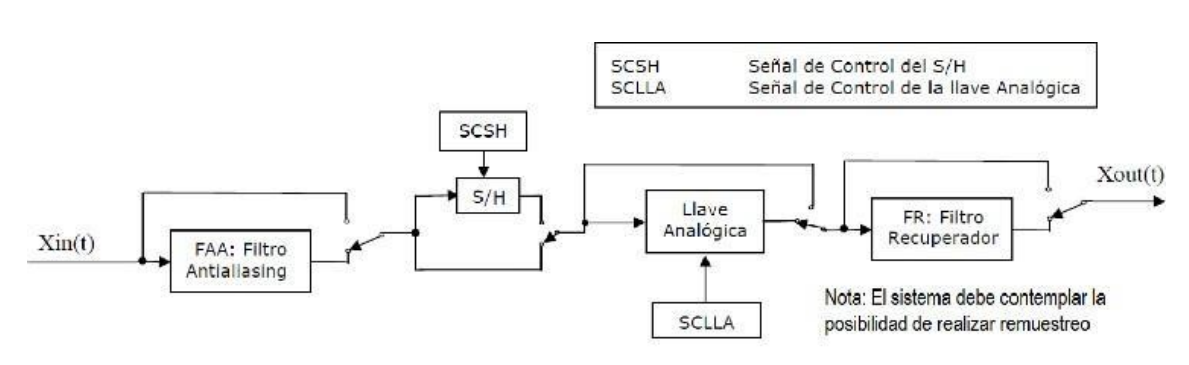
\includegraphics[width=0.8\textwidth]{Imagenes/Circuito_Muestreo.png}
    \caption{Circuito de Muestreo y Retención}
    \label{fig:Circuito_Muestreo}
\end{figure}
Esta implementación del circuito de muestreo y recuperación de la señal analógica nos permite analizar 
los efectos de las distintas etapas del proceso de muestreo y su importancia en el sampleo de la señal.
\subsection{Filtros Pasabajos}
holahola

\subsection{Oscilador}
En la Fig. \ref{esquematico_oscilador} se muestra el oscilador implementado. El circuito utiliza un temporizador NE555 configurado como generador de impulsos, cuya salida se integra mediante una red RC (R1, potenciómetro y C1) para obtener una señal triangular. La frecuencia de oscilación puede ajustarse modificando la resistencia efectiva en el integrador, lo cual se logra a través de un preset en serie con R1. De esta forma, es posible alcanzar frecuencias de oscilación de hasta aproximadamente $200kHz$.

La señal triangular se aplica luego a dos comparadores implementados con amplificadores operacionales TL082. Estos comparadores se configuran como disparadores de Schmitt, de manera que la histéresis de conmutación puede ajustarse con un preset independiente. Este control permite desplazar los umbrales de conmutación de la señal triangular, modificando así el ciclo de trabajo (\textit{duty cycle}) de la onda cuadrada resultante. En la práctica, el rango de variación obtenido es amplio, abarcando aproximadamente entre 5\% y 95\%.

En resumen, el diseño cumple con los requerimientos planteados: generar una señal cuadrada con frecuencia ajustable y con \textit{duty cycle} variable de forma independiente, empleando un oscilador basado en el NE555, un integrador RC y comparadores con histéresis.
\begin{figure}[H]
    \centering
    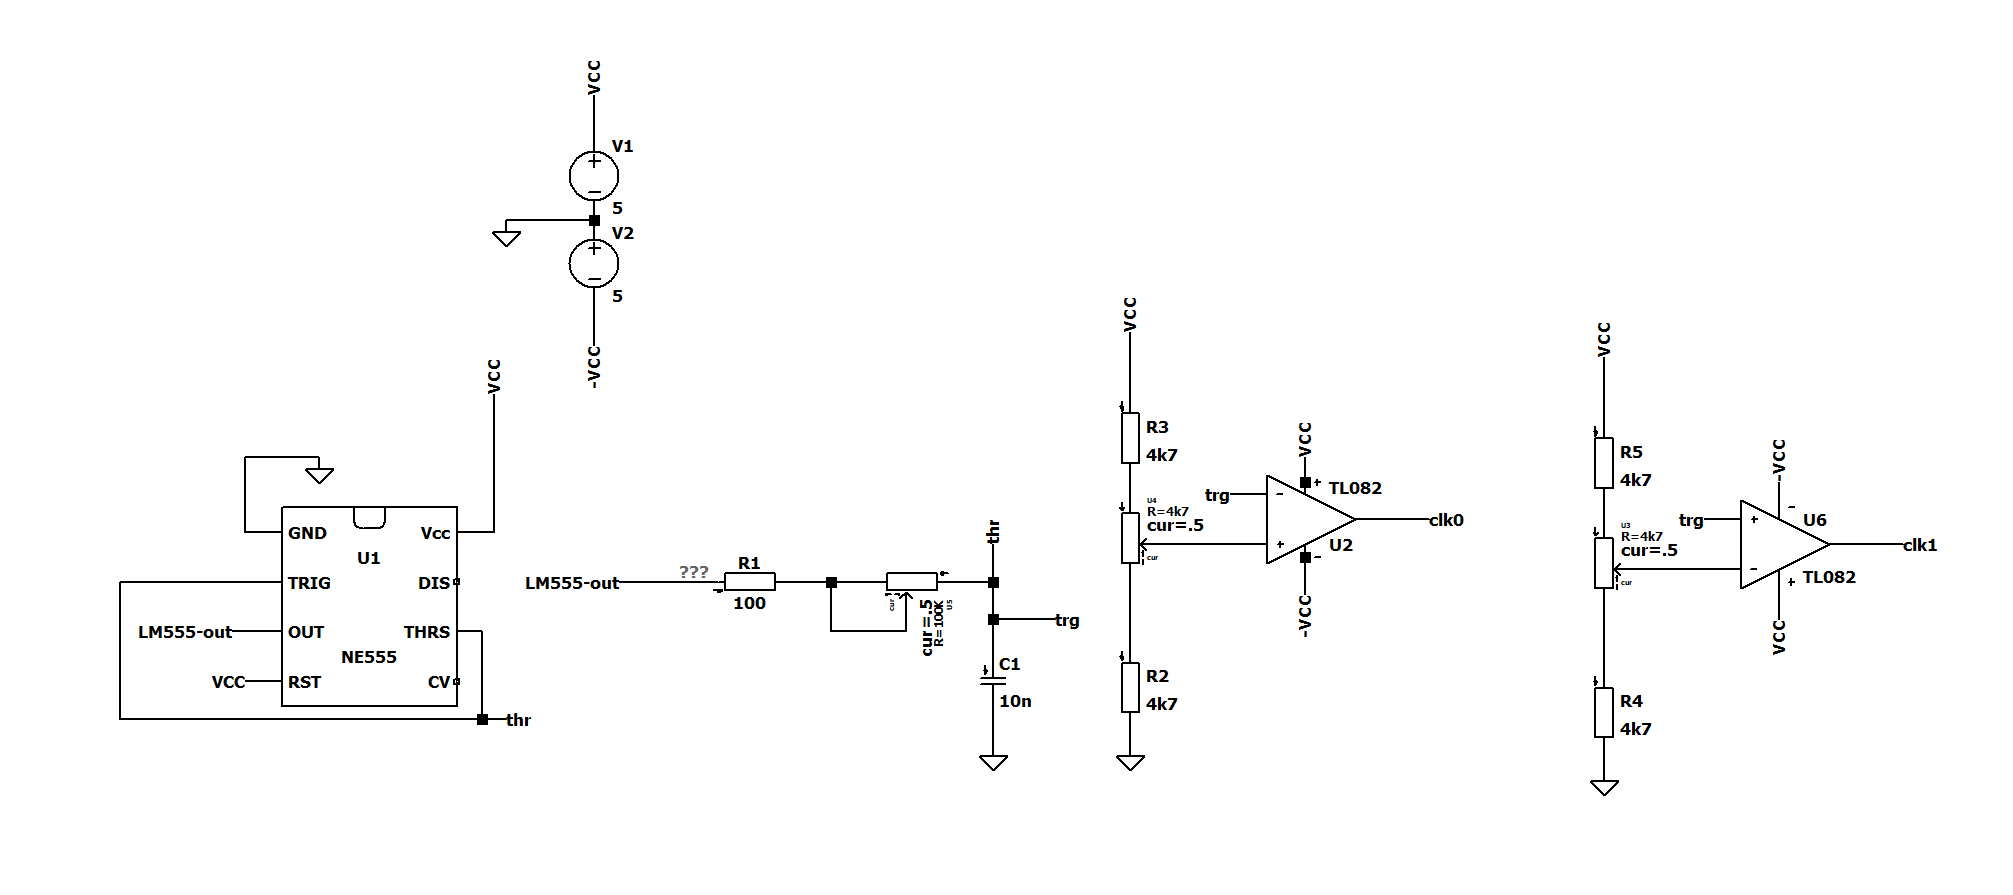
\includegraphics[width=0.8\textwidth]{Imagenes/esquematico_oscilador.png}
    \caption{Esquemático del Oscilador}
    \label{esquematico_oscilador}
\end{figure}
\subsection{Obtención de Señal Muestreada}

